{
\setbeamertemplate{navigation symbols}{}
\setbeamercolor{background canvas}{bg={black}}
\color{white}
\begin{frame}[plain]
\fontsize{36pt}{36pt}\selectfont
\center
\begin{center}
Refactored Level Sets
\newline
\end{center}

\fontsize{12pt}{12pt}\selectfont
Insight Software Consortium\\
Megason Lab, Department of Systems Biology, Harvard Medical School
\newline
\begin{tabular}{cp{.3\textwidth}p{.3\textwidth}p{.3\textwidth}c}
% &
% \centering\includegraphics[height=2cm]{arnaud} &
% \centering\includegraphics[height=2cm]{kishore} &
% \centering\includegraphics[height=2cm]{sean} & \\
\\
\\
&
\centering{}Arnaud Gelas &
\centering{}Kishore Mosaliganti &
\centering{}Sean Megason & \\
\end{tabular}
\end{frame}
}

%\section{Introduction}
\centeredlargetext{black}{white}{
Introduction
}

%%%%%%%%%%%%%%%%%%%%%%%%%%%%%%%%%%%%%%%%%%%%%%%%%%%%%%%%%%%%%%%%%%%%%%%%%%%%%%%%
%%%%%%%%%%%%%%%%%%%%%%%%%%%%%%%%%%%%%%%%%%%%%%%%%%%%%%%%%%%%%%%%%%%%%%%%%%%%%%%%
%%%%%%%%%%%%%%%%%%%%%%%%%%%%%%%%%%%%%%%%%%%%%%%%%%%%%%%%%%%%%%%%%%%%%%%%%%%%%%%%

\begin{frame}
\frametitle{What is a level-set function?}
\begin{columns}
\column{0.4\textwidth}
  \begin{block}
  \begin{itemize}
  \item Implicit function $\phi : \Omega \rightarrow \mathbb{R}$
  \item If $\phi(p) = 0$, $p$ is on the interface $\Gamma$
  \item If $\phi(p) < 0$, $p$ is inside
  \item Else $p$ is outside
  \end{itemize}
  \end{block}
% \column{0.4\textwidth}
% \begin{center}
%  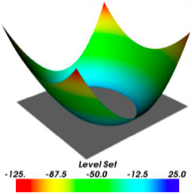
\includegraphics{IntroLevelSet.png}
 % IntroLevelSet.png: 192x194 pixel, 72dpi, 6.77x6.84 cm, bb=0 0 192 194
% \end{center}

\begin{columns}
\end{frame}

%%%%%%%%%%%%%%%%%%%%%%%%%%%%%%%%%%%%%%%%%%%%%%%%%%%%%%%%%%%%%%%%%%%%%%%%%%%%%%%%
%%%%%%%%%%%%%%%%%%%%%%%%%%%%%%%%%%%%%%%%%%%%%%%%%%%%%%%%%%%%%%%%%%%%%%%%%%%%%%%%
%%%%%%%%%%%%%%%%%%%%%%%%%%%%%%%%%%%%%%%%%%%%%%%%%%%%%%%%%%%%%%%%%%%%%%%%%%%%%%%%

\begin{frame}
\frametitle{Level-Set Evolution}
\begin{itemize}
  \item Deforms the level-set function
  \begin{itemize}
    \item Driven by given PDE
    \begin{enumerate}
      \item<2->[yo1]
      \begin{equation*}
      \frac{\partial \phi}{\partial \tau} = 
      \alpha \cdot \overrightarrow{A}(p) \bullet \overrightarrow{\nabla} \phi +
      \gamma \cdot \text{div}\left( \frac{\overrightarrow{\nabla}
      \phi}{\|\overrightarrow{\nabla} \phi\|} \right) \cdot
    \|\overrightarrow{\nabla}
      \phi\|
      \end{equation*}
      \only<2>{
      \begin{columns}
        \column{0.3\textwidth}
        \begin{block}{Advection}
        \begin{center}
          $\alpha \cdot \overrightarrow{A}(p) \bullet \overrightarrow{\nabla}
\phi$ \\
        \end{center}
        $\alpha$: coefficient\\
        $A(p)$: Advection field
        \end{block}

        \column{0.3\textwidth}
        \begin{block}{Curvature}
        \begin{center}
          $\gamma \cdot \|\overrightarrow{\nabla} \phi\| \cdot 
            \text{div}\ \frac{\overrightarrow{\nabla}
            \phi}{\|\overrightarrow{\nabla} \phi\|}$\\
        \end{center}
          $\gamma$: coefficient
        \end{block}
      \end{columns}
    }

      \item<3->[yo2]
      \begin{equation*}
      \frac{\partial \phi}{\partial \tau} = 
      \alpha \cdot P(p) \cdot \|\overrightarrow{\nabla} \phi \| +
      \gamma \cdot \text{div}\left( \frac{\overrightarrow{\nabla}
      \phi}{\|\overrightarrow{\nabla} \phi\|} \right) \cdot
    \|\overrightarrow{\nabla}
      \phi\|
      \end{equation*}
      \only<3>{
      \begin{columns}
        \column{0.3\textwidth}
        \begin{block}<3>{Propagation}
          \begin{center}
          $\beta \cdot P(p) \cdot \|\overrightarrow{\nabla} \phi\|$ \\
          \end{center}
          $\beta$: coefficient \\
          $P(p)$: Propagation field
        \end{block}

        \column{0.3\textwidth}
        \begin{block}{Curvature}
          \begin{center}
          $\gamma \cdot \|\overrightarrow{\nabla} \phi\| \cdot 
            \text{div}\ \frac{\overrightarrow{\nabla}
            \phi}{\|\overrightarrow{\nabla} \phi\|}$\\
          \end{center}
          $\gamma$: coefficient
        \end{block}
      \end{columns}
      }
      \item<4->[Chan and Vese]
      \begin{equation*}
      \frac{\partial \phi}{\partial \tau} = \delta_{\epsilon}(\phi) 
      \left(
      - \lambda_{in} \left( I - \mu_{in} \right) + 
      \lambda_{out} \left( I - \mu_{out} \right)
      \right)
      \end{equation*}
      \only<4>{
      \begin{columns}
        \column{0.3\textwidth}
        \begin{block}{Chan And Vese Internal}
          \begin{center}
          $\delta_{\epsilon}(\phi) \left( \lambda_{in} \left( I - \mu_{in}
\right)\right)$ \\
          \end{center}
          $\lambda_{in}$: coefficient \\
          $\mu_{in}$: Internal Mean
        \end{block}

        \column{0.3\textwidth}
        \begin{block}{Chan And Vese External}
          \begin{center}
          $\delta_{\epsilon}(\phi) \left( \lambda_{out} \left( I - \mu_{out}
\right)\right)$ \\
          \end{center}
          $\lambda_{out}$: coefficient \\
          $\mu_{out}$: External Mean
        \end{block}
      \end{columns}
      }
    \end{enumerate}
  \end{itemize}
\end{itemize}
\end{frame}

%%%%%%%%%%%%%%%%%%%%%%%%%%%%%%%%%%%%%%%%%%%%%%%%%%%%%%%%%%%%%%%%%%%%%%%%%%%%%%%%
%%%%%%%%%%%%%%%%%%%%%%%%%%%%%%%%%%%%%%%%%%%%%%%%%%%%%%%%%%%%%%%%%%%%%%%%%%%%%%%%
%%%%%%%%%%%%%%%%%%%%%%%%%%%%%%%%%%%%%%%%%%%%%%%%%%%%%%%%%%%%%%%%%%%%%%%%%%%%%%%%

\begin{frame}
\frametitle{Level-Set Evolution}
\begin{itemize}
  \item Iterative computation
  \item Topological flexibility
\end{itemize}
\end{frame}


%%%%%%%%%%%%%%%%%%%%%%%%%%%%%%%%%%%%%%%%%%%%%%%%%%%%%%%%%%%%%%%%%%%%%%%%%%%%%%%%
%%%%%%%%%%%%%%%%%%%%%%%%%%%%%%%%%%%%%%%%%%%%%%%%%%%%%%%%%%%%%%%%%%%%%%%%%%%%%%%%
%%%%%%%%%%%%%%%%%%%%%%%%%%%%%%%%%%%%%%%%%%%%%%%%%%%%%%%%%%%%%%%%%%%%%%%%%%%%%%%%

\begin{frame}
\frametitle{Level Sets: Challenges in Segmentation?}
\begin{itemize}
  \item PDE Term choice
    \begin{itemize}
      \item Advection terms ?
      \item Propagation terms ?
      \item Region terms ?
      \item Regularization terms ?
    \end{itemize}
  \item<2-> Stopping criterion
    \begin{itemize}
      \item Number of Iterations ?
      \item Variation of interface length / area ?
      \item Variation of shape area / volume ?
    \end{itemize}
  \item<3-> PDE Parameters tuning
\end{itemize}
\end{frame}

%%%%%%%%%%%%%%%%%%%%%%%%%%%%%%%%%%%%%%%%%%%%%%%%%%%%%%%%%%%%%%%%%%%%%%%%%%%%%%%%
%%%%%%%%%%%%%%%%%%%%%%%%%%%%%%%%%%%%%%%%%%%%%%%%%%%%%%%%%%%%%%%%%%%%%%%%%%%%%%%%
%%%%%%%%%%%%%%%%%%%%%%%%%%%%%%%%%%%%%%%%%%%%%%%%%%%%%%%%%%%%%%%%%%%%%%%%%%%%%%%%

\section{Overview of the Level-Sets in ITKv4}
\centeredlargetext{white}{black}{
Overview of the Level-Sets in ITKv4
}

%%%%%%%%%%%%%%%%%%%%%%%%%%%%%%%%%%%%%%%%%%%%%%%%%%%%%%%%%%%%%%%%%%%%%%%%%%%%%%%%
%%%%%%%%%%%%%%%%%%%%%%%%%%%%%%%%%%%%%%%%%%%%%%%%%%%%%%%%%%%%%%%%%%%%%%%%%%%%%%%%
%%%%%%%%%%%%%%%%%%%%%%%%%%%%%%%%%%%%%%%%%%%%%%%%%%%%%%%%%%%%%%%%%%%%%%%%%%%%%%%%

\begin{frame}
\frametitle{Level Sets Representation}
\begin{itemize}
  \item Discrete
  \begin{itemize}
    \item Dense     *********** Images
    \item Sparse 
    \begin{enumerate}
      \item Whitaker  *********** Images 
      \item Shi       *********** Images 
      \item Malcolm   *********** Images 
    \end{enumerate}
  \end{itemize}
  \item Parametric
  \begin{itemize}
    \item Easy integration of new representation
  \end{itemize}
\end{itemize}
\end{frame}

%%%%%%%%%%%%%%%%%%%%%%%%%%%%%%%%%%%%%%%%%%%%%%%%%%%%%%%%%%%%%%%%%%%%%%%%%%%%%%%%
%%%%%%%%%%%%%%%%%%%%%%%%%%%%%%%%%%%%%%%%%%%%%%%%%%%%%%%%%%%%%%%%%%%%%%%%%%%%%%%%
%%%%%%%%%%%%%%%%%%%%%%%%%%%%%%%%%%%%%%%%%%%%%%%%%%%%%%%%%%%%%%%%%%%%%%%%%%%%%%%%

\begin{frame}
\frametitle{Level Sets Equation}

\begin{columns}
  \column{0.47\textwidth} 
  \begin{block}{Term}
    \begin{itemize}
      \item Contribution for $\phi$ evolution
      \item Contribution for time step computation
      \item Coefficient
    \end{itemize} 
  \alert<2->{Easy to contribute new terms!}
  \end{block}

  \column{0.47\textwidth}
  \begin{block}<3->{TermContainer}
    \begin{itemize}
      \item Represent a given PDEs
      \item Mix of any term
      \item Independant of the representation
    \end{itemize}
  \alert<4->{Easy to contribute new PDEs!}
  \end{block}

\end{columns}

\end{frame}

%%%%%%%%%%%%%%%%%%%%%%%%%%%%%%%%%%%%%%%%%%%%%%%%%%%%%%%%%%%%%%%%%%%%%%%%%%%%%%%%
%%%%%%%%%%%%%%%%%%%%%%%%%%%%%%%%%%%%%%%%%%%%%%%%%%%%%%%%%%%%%%%%%%%%%%%%%%%%%%%%
%%%%%%%%%%%%%%%%%%%%%%%%%%%%%%%%%%%%%%%%%%%%%%%%%%%%%%%%%%%%%%%%%%%%%%%%%%%%%%%%

\begin{frame}
\frametitle{Title}
  \begin{itemize}
    \item N Level-Sets function evolving at the same time
    \item Geometrical Constraints
  \end{itemize}
\end{frame}

%%%%%%%%%%%%%%%%%%%%%%%%%%%%%%%%%%%%%%%%%%%%%%%%%%%%%%%%%%%%%%%%%%%%%%%%%%%%%%%%
%%%%%%%%%%%%%%%%%%%%%%%%%%%%%%%%%%%%%%%%%%%%%%%%%%%%%%%%%%%%%%%%%%%%%%%%%%%%%%%%
%%%%%%%%%%%%%%%%%%%%%%%%%%%%%%%%%%%%%%%%%%%%%%%%%%%%%%%%%%%%%%%%%%%%%%%%%%%%%%%%
\section{Example}
\centeredlargetext{white}{black}{
Example
}

\begin{frame}
  \frametitle{Create a level-set function from binary mask}
  \lstlistingwithnumber{87}{94}{SingleLevelSetWhitaker.cxx}
  \lstlistingwithnumber{98}{100}{SingleLevelSetWhitaker.cxx}
\end{frame}

%%%%%%%%%%%%%%%%%%%%%%%%%%%%%%%%%%%%%%%%%%%%%%%%%%%%%%%%%%%%%%%%%%%%%%%%%%%%%%%%
%%%%%%%%%%%%%%%%%%%%%%%%%%%%%%%%%%%%%%%%%%%%%%%%%%%%%%%%%%%%%%%%%%%%%%%%%%%%%%%%
%%%%%%%%%%%%%%%%%%%%%%%%%%%%%%%%%%%%%%%%%%%%%%%%%%%%%%%%%%%%%%%%%%%%%%%%%%%%%%%%

\begin{frame}
  \frametitle{Create a domain for the level-set function}
  \lstlistingwithnumber{106}{110}{SingleLevelSetWhitaker.cxx}
  \lstlistingwithnumber{114}{125}{SingleLevelSetWhitaker.cxx}
\end{frame}

%%%%%%%%%%%%%%%%%%%%%%%%%%%%%%%%%%%%%%%%%%%%%%%%%%%%%%%%%%%%%%%%%%%%%%%%%%%%%%%%
%%%%%%%%%%%%%%%%%%%%%%%%%%%%%%%%%%%%%%%%%%%%%%%%%%%%%%%%%%%%%%%%%%%%%%%%%%%%%%%%
%%%%%%%%%%%%%%%%%%%%%%%%%%%%%%%%%%%%%%%%%%%%%%%%%%%%%%%%%%%%%%%%%%%%%%%%%%%%%%%%

\begin{frame}
  \frametitle{Setting up the level-set container}
  \lstlistingwithnumber{129}{135}{SingleLevelSetWhitaker.cxx}
  \lstlistingwithnumber{137}{144}{SingleLevelSetWhitaker.cxx}
\end{frame}

%%%%%%%%%%%%%%%%%%%%%%%%%%%%%%%%%%%%%%%%%%%%%%%%%%%%%%%%%%%%%%%%%%%%%%%%%%%%%%%%
%%%%%%%%%%%%%%%%%%%%%%%%%%%%%%%%%%%%%%%%%%%%%%%%%%%%%%%%%%%%%%%%%%%%%%%%%%%%%%%%
%%%%%%%%%%%%%%%%%%%%%%%%%%%%%%%%%%%%%%%%%%%%%%%%%%%%%%%%%%%%%%%%%%%%%%%%%%%%%%%%

\begin{frame}
  \frametitle{Setting up the level-set container}
  \lstlistingwithnumber{129}{135}{SingleLevelSetWhitaker.cxx}
  \lstlistingwithnumber{137}{144}{SingleLevelSetWhitaker.cxx}
\end{frame}

%%%%%%%%%%%%%%%%%%%%%%%%%%%%%%%%%%%%%%%%%%%%%%%%%%%%%%%%%%%%%%%%%%%%%%%%%%%%%%%%
%%%%%%%%%%%%%%%%%%%%%%%%%%%%%%%%%%%%%%%%%%%%%%%%%%%%%%%%%%%%%%%%%%%%%%%%%%%%%%%%
%%%%%%%%%%%%%%%%%%%%%%%%%%%%%%%%%%%%%%%%%%%%%%%%%%%%%%%%%%%%%%%%%%%%%%%%%%%%%%%%

\begin{frame}
  \frametitle{Creating PDE Terms}
  \begin{itemize}
    \item Chan and Vese internal term
    \lstlistingwithnumber{151}{158}{SingleLevelSetWhitaker.cxx}
    \item Chan and Vese external term
    \lstlistingwithnumber{162}{169}{SingleLevelSetWhitaker.cxx}
  \end{itemize}
\end{frame}

%%%%%%%%%%%%%%%%%%%%%%%%%%%%%%%%%%%%%%%%%%%%%%%%%%%%%%%%%%%%%%%%%%%%%%%%%%%%%%%%
%%%%%%%%%%%%%%%%%%%%%%%%%%%%%%%%%%%%%%%%%%%%%%%%%%%%%%%%%%%%%%%%%%%%%%%%%%%%%%%%
%%%%%%%%%%%%%%%%%%%%%%%%%%%%%%%%%%%%%%%%%%%%%%%%%%%%%%%%%%%%%%%%%%%%%%%%%%%%%%%%

\begin{frame}
  \frametitle{Setting up PDE}
  \lstlistingwithnumber{174}{178}{SingleLevelSetWhitaker.cxx}
  \lstlistingwithnumber{180}{182}{SingleLevelSetWhitaker.cxx}
  \lstlistingwithnumber{184}{185}{SingleLevelSetWhitaker.cxx}
  \lstlistingwithnumber{188}{191}{SingleLevelSetWhitaker.cxx}
\end{frame}

%%%%%%%%%%%%%%%%%%%%%%%%%%%%%%%%%%%%%%%%%%%%%%%%%%%%%%%%%%%%%%%%%%%%%%%%%%%%%%%%
%%%%%%%%%%%%%%%%%%%%%%%%%%%%%%%%%%%%%%%%%%%%%%%%%%%%%%%%%%%%%%%%%%%%%%%%%%%%%%%%
%%%%%%%%%%%%%%%%%%%%%%%%%%%%%%%%%%%%%%%%%%%%%%%%%%%%%%%%%%%%%%%%%%%%%%%%%%%%%%%%

\begin{frame}
  \frametitle{Stopping criterion}
  \lstlistingwithnumber{193}{196}{SingleLevelSetWhitaker.cxx}
\end{frame}

%%%%%%%%%%%%%%%%%%%%%%%%%%%%%%%%%%%%%%%%%%%%%%%%%%%%%%%%%%%%%%%%%%%%%%%%%%%%%%%%
%%%%%%%%%%%%%%%%%%%%%%%%%%%%%%%%%%%%%%%%%%%%%%%%%%%%%%%%%%%%%%%%%%%%%%%%%%%%%%%%
%%%%%%%%%%%%%%%%%%%%%%%%%%%%%%%%%%%%%%%%%%%%%%%%%%%%%%%%%%%%%%%%%%%%%%%%%%%%%%%%

\begin{frame}
  \frametitle{Starts the evolution}
  \begin{itemize}
    \item Set a stopping criterion
    \lstlistingwithnumber{193}{196}{SingleLevelSetWhitaker.cxx}
    \item Evolve
    \lstlistingwithnumber{198}{204}{SingleLevelSetWhitaker.cxx}
    \lstlistingwithnumber{208}{208}{SingleLevelSetWhitaker.cxx}
  \end{itemize}
\end{frame}

%%%%%%%%%%%%%%%%%%%%%%%%%%%%%%%%%%%%%%%%%%%%%%%%%%%%%%%%%%%%%%%%%%%%%%%%%%%%%%%%
%%%%%%%%%%%%%%%%%%%%%%%%%%%%%%%%%%%%%%%%%%%%%%%%%%%%%%%%%%%%%%%%%%%%%%%%%%%%%%%%
%%%%%%%%%%%%%%%%%%%%%%%%%%%%%%%%%%%%%%%%%%%%%%%%%%%%%%%%%%%%%%%%%%%%%%%%%%%%%%%%

\section{Exercice 1}
\centeredlargetext{white}{black}{
Add a curvature term to the example
}

%%%%%%%%%%%%%%%%%%%%%%%%%%%%%%%%%%%%%%%%%%%%%%%%%%%%%%%%%%%%%%%%%%%%%%%%%%%%%%%%
%%%%%%%%%%%%%%%%%%%%%%%%%%%%%%%%%%%%%%%%%%%%%%%%%%%%%%%%%%%%%%%%%%%%%%%%%%%%%%%%
%%%%%%%%%%%%%%%%%%%%%%%%%%%%%%%%%%%%%%%%%%%%%%%%%%%%%%%%%%%%%%%%%%%%%%%%%%%%%%%%

\section{Exercice 2}
\centeredlargetext{white}{black}{
Change the represesentation from Whitaker's to Shi's
}

\begin{frame}
\frametitle{Wrap-up}
\begin{itemize}
  \item Send us feedback (good or bad)
  \begin{itemize}
    \item \url{arnaud_gelas@hms.harvard.edu} 
    \item \url{kishore_mosaliganti@hms.harvard.edu} 
    \item \url{sean_megason@hms.harvard.edu}
  \end{itemize}
%   \item Raffle\\
% \includegraphics[height=1.5in]{asus}
\end{itemize}
\end{frame}

